%\documentclass[11pt,aspectratio=169]{beamer}
\documentclass[11pt,aspectratio=169,handout]{beamer}

\usepackage{amsmath}
\usepackage{amsfonts}
\usepackage{amssymb}
\usepackage{graphbox}
\usepackage{sgamevar}
\usepackage{pgfplots}
\usepackage{tikz}
\usepackage{pstricks,pst-node}
\usepackage{bigdelim}
\usepackage{qrcode}
\usepackage[absolute,overlay]{textpos}
\usepackage[ruled,vlined]{algorithm2e}



% alg
\SetKwFor{Repeat}{repeat}{}{}
\SetKwComment{Comment}{$\triangleright$ }{}
\SetCommentSty{textsf}
% pgfplot settings
\usepgfplotslibrary{fillbetween}

% tikz settings
\tikzset{
    invisible/.style={text opacity=1,opacity=0},
    visible on/.style={alt=#1{}{invisible}},
    alt/.code args={<#1>#2#3}{%
      \alt<#1>{\pgfkeysalso{#2}}{\pgfkeysalso{#3}}
    },
  }
\newcommand{\nebox}[2][]{\tikz[baseline=(h.base)]\node[rounded corners,rectangle,draw,line width=0.7pt,text depth=-4.9pt,#1] (h) {#2};}
\usetikzlibrary{arrows}
% Customized colors

\definecolor{ashgrey}{rgb}{0.7, 0.75, 0.71}
\definecolor{lightblue}{RGB}{140, 201, 247}
\definecolor{darkgreen}{RGB}{113, 160, 55}
\definecolor{darkblue}{RGB}{78, 103, 200}
\definecolor{darkpurple}{RGB}{112, 48, 160}

% Hyperlink settings

\hypersetup{colorlinks,urlcolor=darkgreen}

%Beamer settings

\setbeamertemplate{navigation symbols}{} 
\setbeamertemplate{footline}[frame number]
\setbeamertemplate{itemize items}[circle]
\setbeamertemplate{section in toc}[sections numbered]
\setbeamertemplate{subsection in toc}[subsection numbered]

\setbeamercolor{section in toc}{fg=blue}

\AtBeginSection[ ]{
 \begin{frame}{Outline}
  \hypersetup{linkcolor=black}
  \tableofcontents[currentsection]
 \end{frame}
}

% Graphics settings

\graphicspath{{../Figures/}}

% PGFPlot settings

\pgfplotsset{compat = newest}

% Gamesvar settings

\setlength{\arrayrulewidth}{0.91pt}
\renewcommand{\gamestretch}{1.68}
\def\stackedpayoffs#1#2{%
 \begin{array}{c}#1\\[2mm]#2\end{array}
}

% Math

\DeclareMathOperator*{\argmax}{argmax}
\DeclareMathOperator*{\argmin}{argmin}

\newcommand\given[1][]{\:#1\vert\:}
\newtheorem{proposition}{Proposition}

% New environments

\newenvironment{itemizes}[1][1em]{
 \vspace{#1}
 \begin{itemize}
 \setlength{\itemsep}{#1}
}{
 \end{itemize}
}


% Shared title frame

\title{Game-theoretic \\ Foundations of Multi-agent Systems}

\author{Seyed Majid Zahedi}
\titlegraphic{\vspace{-4.2em} 
\includegraphics[height=5.8em]{Logos/logo2}}

\date{} 
\subject{Lecture 1} 
\logo{
\includegraphics[height=5.6em]{Logos/logo1}}
\subtitle{\vspace{2.1em}Lecture 3: Games in Normal Form}

\begin{document}

 \begin{frame}[plain]
  \titlepage
 \end{frame}
 
 \section{Normal-form Games: Definition, Notations, and Examples}
 
  \begin{frame}{Normal-form Games}
   \begin{itemize}[<+->]  
   \setlength{\itemsep}{1.5em}
    \item Let's start with games in which all agents act simultaneously
    \item Agents choose their actions without knowledge of other agents' actions
    \item Such games are referred to as \alert{strategic-form games} or \alert{normal-form games}
   \end{itemize}
  \end{frame}
  
    \begin{frame}{Normal-form Games: Definition}
   \begin{itemize}[<+->]
   \setlength{\itemsep}{1.5em}
    \item The game consists of a set of agents, $N=\{1,2,\dots,n\}$
    \item Set of available actions to agent $i$ is denoted by $A_i$
    \item Action taken by agent $i$ is denoted by $a_i \in A_i$
    \item Outcome of game is an \alert{action profile} of all agents, $a = (a_1,\dots,a_n)$
    \item Set of all action profiles is denoted by $A = \prod A_i$
    \item Agent $i$ has a utility function $u_i$ that maps outcomes to real numbers
   \end{itemize}
  \end{frame}
  
  \begin{frame}{Some Notations}
   \begin{itemize}
   \setlength{\itemsep}{1.5em}
    \item $a_{-i} = (a_1,\dots,a_{i-1},a_{i+1},\dots,a_n)$ is an action profile of all agents except $i$
    \item $A_{-i} = \prod_{j\ne i}A_j$ is set of action profiles of all agents except $i$
    \item $a = (a_i,a_{-i}) \in A$ is another way of denoting an action profile (or an outcome)
   \end{itemize}
  \end{frame}
  
  \begin{frame}{Matrix-form Representation}
   \begin{itemize}[<+->]
    \item When $A_i$ is finite for all $i$, we call the game \alert{finite game}
    \item For 2 agents and small action sets, game can be represented in \alert{matrix form}
    \vspace{0.7em}
    \begin{center}
     \hspace{-5.6em}
     \begin{game}{2}{2}[Agent 1][Agent 2]
      	\> x		\> y		\\
      m	\> $a,b$	\> $e,f$	\\
      n	\> $c,d$	\> $g,h$
     \end{game}
    \end{center}
    \vspace{0.7em}
    \item Each cell indexed by  row $r$ and column $c$ contains a pair, $(p,q)$, where $p = u_1(r,c)$ and $q = u_2(r,c)$.
   \end{itemize}
  \end{frame}
 
  \begin{frame}{Example: Matching Pennies}
   \begin{itemize}
    \item Each agent has a penny and independently chooses to display either heads or tails
    \item Agents compare their pennies
    \item<+-> If they are the same, agent 1 pockets both, otherwise agent 2 pockets them
    \begin{center}
     \hspace{-3.5em}
     \begin{game}{2}{2}
      		\> Heads		\> Tails		\\
      Heads	\> $-1,1$	\> $1,-1$	\\
      Tails	\> $1,-1$	\> $-1,1$
     \end{game}
    \end{center}
    \vspace{0.7em}
    \item<+-> \alert{Zero-sum game}: Utility of one agent is negative of utility of other agent
   \end{itemize}
  \end{frame}

  \begin{frame}{Example: Rock, Paper, Scissors Game}
   \begin{itemize}
    \item Three-strategy generalization of the matching-pennies game
    \vspace{1em}
    \begin{center}
     \hspace{-4.9em}
     \begin{game}{3}{3}
      			\> Rock		\> Paper		\> Scissors	\\
      Rock		\> $0,0$		\> $-1,1$	\> $1,-1$	\\
      Paper		\> $1,-1$	\> $0,0$ 	\> $-1,1$	\\
      Scissors	\> $-1,1$	\> $1,-1$	\> $0,0$
     \end{game}
    \end{center}
   \end{itemize}
  \end{frame}    
  
  \begin{frame}{Example: Coordination Game}
   \begin{itemize}
    \item Two drivers driving towards each other in a country with no traffic rules
    \item Drivers must independently decide whether to drive on the left or on the right
    \item<+-> If drivers choose the same side (left or right) they have some high utility, and otherwise they have a low utility
    \begin{center}
     \hspace{-3.5em}
     \begin{game}{2}{2}
      		\> Left		\> Right		\\
      Left	\> $1,1$		\> $-1,-1$	\\
      Right	\> $-1,-1$	\> $1,1$
     \end{game}
    \end{center}
    \vspace{0.7em}
    \item<+-> \alert{Team game}: For all outcomes $s$, and any pair of agents $i$ and $j$, it is the case that $u_i(a) = u_j(a)$ (also known as \alert{common-payoff game} or \alert{pure-coordination game})
   \end{itemize}
  \end{frame}
  
  \begin{frame}{Example: Cournot Competition}
   \begin{itemize}
    \item Two firms producing a homogeneous good for the same market
    \item Action of each firm is the amount of good it produces ($a_i \in [0,\infty]$)
    \item Utility of each firm is its total revenue minus its total cost
     $$u_i(a_1,a_2) = a_i p(a_1 + a_2) - c a_i$$
    \begin{itemize}[<2->]
     \item $p(\cdot)$ is the price function that maps total production to a price
     \item$c$ is a unit cost
     \item E.g., $p(x) = \max(0, 2 - x)$ and $c = 1$
    \end{itemize}
   \end{itemize}
  \end{frame}
  
 \section{Dominant Strategy Equilibrium}
  \begin{frame}{Mixed and Pure Strategies}
   \begin{itemize}[<+->]
    \setlength{\itemsep}{0.56em}
    \item Let $\Delta(X)$ be set of all probability distributions over $X$
    \item Set of \alert{(mixed) strategies} for agent $i$ is denoted by $S_i = \Delta(A_i)$
    \item For mixed strategy $s_i \in S_i$, $s_i(a)$ is probability that action $a$ is played under $s_i$
    \item \alert{Pure strategy} is a mixed strategy that puts probability $1$ on a single action
    \item \alert{Support} of mixed strategy $s_i$ is set of pure strategies, $a_i$, such that $s_i(a_i) > 0$
    \item Expected utility of agent $i$ for a (mixed) \alert{strategy profile} $s = (s_1,\dots,s_n)$ is
     $$u_i(s) = \sum_{a\in A} u_i(a) \prod_{j\in N}s_j(a_j)$$ 
   \end{itemize}
  \end{frame}
  
  \begin{frame}{Example}
   \begin{center}
    \hspace{-1.4em}
    \begin{game}{3}{3}[Agent 1][Agent 2]
     					\> R ($\frac{2}{3}$)	\> P (0)		\> S ($\frac{1}{3}$)	\\
     R ($\frac{1}{3}$)	\> $0,0$				\> $-1,1$	\> $1,-1$			\\
     P ($\frac{2}{3}$)	\> $1,-1$			\> $0,0$		\> $-1,1$			\\
     S (0)				\> $-1,1$			\> $1,-1$	\> $0,0$
    \end{game}
   \end{center}
   \vspace{1.4em}
   \begin{itemize}
    \item $u_1 = 2/9 \times 0 + 1/9 \times 1 + 4/9 \times 1 - 2/9 \times 1 = 1/3$
    \item $u_2 = 2/9 \times 0 - 1/9 \times 1 - 4/9 \times 1+ 2/9 \times 1 = -1/3$
   \end{itemize}
  \end{frame}
  
  \begin{frame}{Dominant and Dominated Strategies}
   \begin{itemize}[<+->]
    \setlength{\itemsep}{0.56em}
    \item Let $s_i$ and $s^\prime_i$ be two strategies of agent $i$
    \item $s_i$ \alert{strictly dominates} $s^\prime_i$ if 
    \begin{itemize}[<.->]
     \item $u_i(s_i, s_{-i}) > u_i(s^\prime_i,s_{-i})$ for all $s_{-i} \in S_{-i}$
    \end{itemize}
    \item $s_i$ \alert{weakly dominates} $s^\prime_i$ if 
    \begin{itemize}[<.->]
     \item $u_i(s_i, s_{-i}) \ge u_i(s^\prime_i,s_{-i})$ for all $s_{-i} \in S_{-i}$, and
     \item  $u_i(s_i, s_{-i}) > u_i(s^\prime_i,s_{-i})$ for at least one $s_{-i} \in S_{-i}$
    \end{itemize}
    \item $s_i$ is strictly/weakly \alert{dominant} if it strictly/weakly dominates all other strategy
    \item $s_i$ is strictly/weakly \alert{dominated} if another strategy strictly/weakly dominates it
    \item $s=(s_1,\dots,s_n)$ is \alert{dominant strategy equilibrium} if $s_i$ is dominant strategy for all $i$
   \end{itemize}
  \end{frame}
  
  \begin{frame}{Example: Prisoner's Dilemma}
   \begin{itemize}
    \item Two prisoners suspected of a crime are taken to separate interrogation rooms
    \item Each can either confess to the crime or deny it
    \begin{center}
     \hspace{-3.5em}
     \begin{game}{2}{2}
      	\> D			\> C			\\
      D	\> $-2,-2$	\> $-4,-1$	\\
      C	\> $-1,-4$	\> $-3,-3$
     \end{game}
    \end{center}
    \vspace{0.7em}
    \item<+-> Absolute value of utilities are the length of jail term each prisoner gets
    \item<+-> Confess is strictly dominant strategy for both prisoners
    \item<+-> (C,C) is a strict dominant strategy equilibrium
    \item<+-> The dilemma: (D,D) is better for both prisoners, but they won't play it!
   \end{itemize}
  \end{frame}
  
  \begin{frame}{Iterated Elimination of Strictly Dominated Strategies}
   \begin{itemize}
    \sgcolsep=0.3em
    \item<1-> All \alert{strictly dominated pure strategies} can be ignored
    \vspace{0.49em}
    \begin{center}
     \small
     \hspace{-3.5em}
     \visible<2->{
      \begin{game}{3}{3}
       	\> L		\> C		\> R 	\\
       U	\> $3,1$	\> $0,2$	\> $0,0$	\\
       M	\> $1,2$	\> $1,1$	\> $5,0$	\\
       D	\> $0,1$	\> $4,2$	\> $0,0$
      \end{game}
     }
     \hspace{-0.77em}
     \visible<4->{
      \raisebox{-0.91em}{$\Rightarrow$}
      %\hspace{0.28em}
      \begin{game}{3}{2}
       	\> L		\> C		\\
       U	\> $3,1$	\> $0,2$	\\
       M	\> $1,2$	\> $1,1$	\\
       D	\> $0,1$	\> $4,2$	
      \end{game}
     }
     \hspace{-0.77em}
     \visible<6->{      
      \raisebox{-0.91em}{$\Rightarrow$}
      %\hspace{0.28em}
      \begin{game}{2}{2}
      	\> L		\> C		\\
       U	\> $3,1$	\> $0,2$	\\
       D	\> $0,1$	\> $4,2$	
      \end{game}
     }
     \hspace{-0.77em}
     \visible<8->{
      \raisebox{-0.91em}{$\Rightarrow$}
      %\hspace{0.28em}
      \begin{game}{2}{1}
      	\> C		\\
       U	\> $0,2$	\\
       D	\> $4,2$
      \end{game}
     }
     \hspace{-0.77em}
     \visible<9->{
      \raisebox{-0.91em}{$\Rightarrow$}
      %\hspace{0.28em}
      \begin{game}{1}{1}
      	\> C		\\
       D	\> $4,2$
      \end{game}
     }
    \end{center}
    \vspace{0.7em}
    \item<3-> Column R can be eliminated, since it is dominated by, for example, column L
    \item<5-> M is not dominated by U or D but is dominated by 0.5U + 0.5D mixed strategy
    \item<7-> Note, however, that it was not dominated before the elimination of the R column
   \end{itemize}
  \end{frame}
  
  \begin{frame}{Iterated Elimination of Strictly Dominated Strategies (cont.)}
   \begin{itemize}[<+->]
    \setlength{\itemsep}{1em}
    \item Once one pure strategy is eliminated, another strategy that was not dominated can become dominated
    \item In finite games, iterated elimination of strictly dominated strategies ends after finite number of iterations
    \item Order of elimination does not matter when removing strictly dominated strategies (\alert{Church–Rosser property})
    \item Elimination order can make a difference in final outcome when removing weakly dominated strategies
    \item If the procedure ends with a single strategy for each agent, then the game is said to be \alert{dominance solvable}
   \end{itemize}
  \end{frame}
  
  \begin{frame}{Existence of Dominant Strategy Equilibrium}
   \begin{itemize}[<+->]
    \item Dominant strategy equilibrium does not always exist
    \item Example: Matching pennies
    \begin{center}
     \hspace{-3.5em}
     \begin{game}{2}{2}
      		\> Heads		\> Tails		\\
      Heads	\> $-1,1$	\>	$1,-1$	\\
      Tails	\> $1,-1$	\> $-1,1$
     \end{game}
    \end{center}
   \end{itemize}
  \end{frame}
  
 \section{Nash Equilibrium}
  \begin{frame}{Best Response}
   \begin{itemize}[<+->]
    \setlength{\itemsep}{0.49em}
    \item Picking a strategy would be simple if an agent knew how others were going to act
    \item \alert{Best response}: $s^{*}_{i}\in BR_{i}(s_{-i})$ iff $u_i(s^{*}_i , s_{-i}) \ge u_i(s_i, s_{-i})$ for all strategies $s_i \in S_i$
    \item Best response \alert{is not} necessarily unique
    \begin{itemize}[<.->]
     \item If there is more than one best response, any mixed strategy over those must be a best response as well
    \end{itemize}
    \item Best response is not a \alert{solution concept}
    \begin{itemize}[<.->]
     \item I.e., it does not identify an interesting set of outcomes
     \item Because agents do not know what strategies others will play 
    \end{itemize}
    \item However, we can leverage the idea of best response to define what is arguably the most central notion in game theory, the \alert{Nash equilibrium}
   \end{itemize}
  \end{frame}

  \begin{frame}{Nash Equilibrium - Intersection of Best Responses}
   \begin{columns}
    \begin{column}{0.72\textwidth}
     \begin{itemize}[<+->]
      \setlength{\itemsep}{0.7em}
      \item $s^{*} = (s^{*}_1,...,s^{*}_n)$ is a \alert{Nash equilibrium} iff $\forall i, ~ s^{*}_{i} \in Br_i(s^{*}_{-i})$
      \item No agent can profitably deviate given strategies of others
      \item Nash equilibrium  is a \alert{stable} strategy profile
      \item \alert{Nash theorem}: Every \underline{finite game} has a Nash equilibrium
     \end{itemize}
    \end{column}
    \begin{column}{0.28\textwidth}
     \begin{center}
      \includegraphics<5->[align=c,vshift=-6.3em,height=0.49\paperheight]{L3/bm}%
      \llap{\includegraphics<6->[align=c, vshift=-7.7em,height=0.56\paperheight]{L3/Nash}}
     \end{center}
    \end{column}
   \end{columns} 
  \end{frame}
  
  \begin{frame}{Example: Battle of Sexes}
   \begin{itemize}
    \item Husband and wife wish to meet this evening, but have a choice between two events to attend: football or opera
    \item Husband would prefer to go to football, wife would prefer opera
    \item Both would prefer to go to the same event rather than different ones
    \vspace{1em}
    \begin{center}
     \hspace{-9.8em}
     \begin{game}{2}{2}[Husband][Wife]
      			\> Football	\> Opera		\\
      Football	\>	\only<1-5>{\alert<2-5>{$2$}$,$\alert<4-5>{$1$}} \only<6->{\nebox[red]{$2,1$}}\>	$0,0$	\\
      Opera		\> $0,0$	\> \only<1-5>{\alert<3-5>{$1$}$,$\alert<5-5>{$2$}} \only<6->{\nebox[red,]{$1,2$}}
     \end{game}
    \end{center}
    \vspace{10pt}
    \item<7> Are these the only Nash equilibria?
   \end{itemize}
  \end{frame}
  
  \begin{frame}{Example: Battle of Sexes (cont.)}
   \begin{center}
    \hspace{-2.8em}
    \begin{game}{2}{2}
  	  		\> F ($p$)	\> O	 ($1-p$)\\
     F		\> $2,1$		\> $0,0$		\\
     O		\> $0,0$		\> $1,2$
    \end{game}
   \end{center}
   \vspace{10pt}
   \begin{itemize}[<+->]
    \item In general, it is tricky to compute mixed-strategy equilibria (will discuss this later)
    \item It becomes easy when we know (or can guess) support of equilibrium strategies
    \item Let us now guess that both agents randomize over both F and O
    \item Wife's strategy is to play F w.p. $p$ and O w.p. $1 - p$
    \item Husband must be indifferent between F and O (why?):
    $$u_H(F) = u_H(O) \Rightarrow 2\times p = (1 - p) \Rightarrow p = 1/3$$
    \item You can show that the unique mixed-strategy NE is $\{(\frac{2}{3}, \frac{1}{3}), (\frac{1}{3}, \frac{2}{3})\}$
   \end{itemize}
  \end{frame}
  
  \begin{frame}{Example: Cournot Competition}
   \begin{columns}
    \begin{column}{0.63\textwidth}
     \begin{itemize}
      \item $u_i(a_1,a_2) = a_i \max(0,2-a_1-a_2) - a_i$
      \item Using first order optimality conditions, we have
      $$
       \begin{aligned}
        BR_i(a_{-i}) & = \argmax_{a_i\ge 0} a_i (2 - a_i - a_{-i}) - a_i & \\
                     & = \begin{cases} 
                          (1-a_{-i})/2  &\text{if } a_{-i} < 1,\\
                          0             &\text{Otherwise}.
   	                     \end{cases}
       \end{aligned}
      $$
     \end{itemize}
    \end{column}
    \begin{column}{0.37\textwidth}
     \begin{center}
      \begin{tikzpicture}
      \begin{axis}[
       width=0.8\textwidth, height=0.8\textwidth,
       axis line style={very thick, line cap=rect,},
       label style={font=\tiny},
       axis x line=bottom, axis y line=left,
       xmin=0, xmax=1.75, ymin=0, ymax=1.75,
       xlabel=$a_1$, ylabel=$a_2$,
       xtick=\empty, ytick=\empty,
       extra x ticks={0.5,1},
       extra x tick labels={1/2,1},
       extra x tick style ={font=\tiny},
       extra y ticks={0.5,1},
       extra y tick labels={1/2,1},
       extra y tick style ={font=\tiny},
       clip=false
      ]
       \only<2->{
        \addplot[red,thick, line cap=round, smooth,domain=0:1]{(1-x)/2};
        \addplot[-stealth,red,thick] coordinates {(1,0) (1.5,0)}
         node [pos=0.5,yshift=8pt] {{\tiny $BR_2$}};
       }
       \only<3->{
        \addplot[blue, thick, line cap=round, smooth,domain=0:0.5]{1-2*x};
        \addplot[-stealth,blue,thick] coordinates {(0,1) (0,1.5)}
         node [pos=0.5,xshift=8pt] {{\tiny $BR_1$}};
       }
      \end{axis}
      \end{tikzpicture}
     \end{center}
    \end{column}
   \end{columns}
  \end{frame}
  
  \begin{frame}{The ''Equilibrium Selection Problem''}
  \begin{itemize}[<+->]
   \item You are about to play a game that you have never played before with a person that you have never met
   \item According to which equilibrium should you play?
   \begin{itemize}
    \item Equilibrium that maximizes the sum of utilities (\alert{social welfare})
    \item Or, at least not a \alert{Pareto-dominated} equilibrium
    \item So-called focal equilibria (e.g., ''Meet in Paris'' game - you and a friend were supposed to meet in Paris at noon on Sunday, but you forgot to discuss where and you cannot communicate. Where will you go?)
    \item Equilibrium that is the convergence point of some learning process
    \item An equilibrium that is easy to compute
    \item $\dots$
   \end{itemize}
   \item Equilibrium selection is a difficult problem
  \end{itemize}
  \end{frame}
  
 \section{Price of Anarchy}

  \begin{frame}{Braess's Paradox}
   \begin{center}
    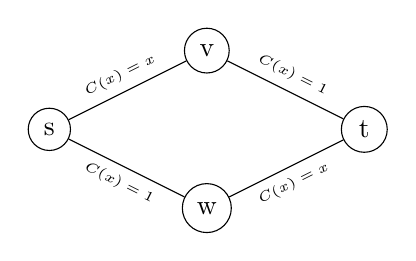
\begin{tikzpicture}
     \node[shape=circle, draw=black] (s) at (0,0)  {s};
     \node[shape=circle, draw=black] (v) at (2,1)  {v};
     \node[shape=circle, draw=black] (w) at (2,-1) {w};
     \node[shape=circle, draw=black] (t) at (4,0)  {t};

     \path (s) edge[above] node[sloped] {\tiny $C(x) = x$} (v);
     \path (s) edge[below] node[sloped] {\tiny $C(x) = 1$} (w);
     \path (v) edge[above] node[sloped] {\tiny $C(x) = 1$} (t);
     \path (w) edge[below] node[sloped] {\tiny $C(x) = x$} (t);
    \end{tikzpicture}
   \end{center}
   \begin{itemize}[<+->]
    \item Suppose there are $2k$ drivers commuting from $s$ to $t$
    \item $C(x)$ indicates travel time in hours for $x$ fraction of drivers 
    \item $k$ drivers going through $v$, and $k$ going through $w$ is NE (why?)
   \end{itemize}
  \end{frame}
  
  \begin{frame}{Braess's Paradox (cont.)}
   \begin{center}
    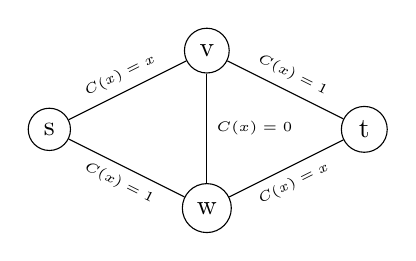
\begin{tikzpicture}
     \node[shape=circle, draw=black] (s) at (0,0)  {s};
     \node[shape=circle, draw=black] (v) at (2,1)  {v};
     \node[shape=circle, draw=black] (w) at (2,-1) {w};
     \node[shape=circle, draw=black] (t) at (4,0)  {t};

     \path (s) edge[above] node[sloped] {\tiny $C(x) = x$} (v);
     \path (s) edge[below] node[sloped] {\tiny $C(x) = 1$} (w);
     \path (v) edge[above] node[sloped] {\tiny $C(x) = 1$} (t);
     \path (w) edge[below] node[sloped] {\tiny $C(x) = x$} (t);

     \path (v) edge[right] node[] {\tiny $C(x) = 0$} (w);
    \end{tikzpicture}
   \end{center}
   \begin{itemize}
    \item Suppose we install a teleportation device allowing instant travel from $v$ to $w$
    \item What is new NE? 
    \item What is optimal commute time?
    \item \alert{Price of anarchy}: ratio between (worst) NE performance and optimal performance
    \begin{itemize}[<+->]
     \item Ratio between 2 and 3/2 in Braess's Paradox
    \end{itemize}
   \end{itemize}
  \end{frame}
  
 \section{Minmax Theorem} 
  \begin{frame}{Maxmin Strategy}
   \begin{itemizes}
    \item \alert{Maxmin strategy} for agent $i$ is 
    $$\underset{s_i}{\argmax} \; \underset{s_{-i}}{\min} \; u_i(s_i,s_{-i})$$
    \item Maxmin value for agent $i$ is 
    $$\underset{s_i}{\max} \; \underset{s_{-i}}{\min} \; u_i(s_i,s_{-i})$$
    \item If $i$ plays maxmin strategy and others play arbitrarily, $i$ still receives expected payoff of at least their maxmin value
   \end{itemizes}
  \end{frame}
  
  \begin{frame}{Example: Battle of Sexes}
   \begin{columns}
    \begin{column}{0.5\textwidth}
     \begin{center}
      \begin{tikzpicture}
       \begin{axis}[
        width=0.8\textwidth, height=0.8\textwidth,
        axis line style={very thick, line cap=rect,},
        label style={font=\tiny},
        axis x line=bottom, axis y line=left,
        xmin=0, xmax=1.25, 
        ymin=0, ymax=2.25,
        xlabel=$p$, ylabel=$u_{W}$,
        xtick=\empty, ytick=\empty,
        extra x ticks={1/3,1},
        extra x tick labels={1/3,1},
        extra x tick style ={font=\tiny},
        extra y ticks={2/3,1,2},
        extra y tick labels={2/3,1,2},
        extra y tick style ={font=\tiny},
        clip=false
       ]
        \only<1-2>{
         \addplot[mark=*,mark options={scale=0.7,black},densely dashed,gray] coordinates {(1,0) (1,2)};
         \addplot[mark=*,mark options={scale=0.7,black},densely dashed,gray] coordinates {(0.,2) (1,2)};
         \addplot[brown,thick, line cap=round, smooth,domain=0:1]{2*x} 
          node [pos=0.8, yshift=10pt, xshift=-10] {{\tiny H plays O}};
        }
        \only<2>{
         \addplot[blue, thick, line cap=round, smooth,domain=0:1]{1-x}
          node [pos=0.8, yshift=15] {{\tiny H plays F}};
        }
        \only<3>{ 
         \addplot[mark=*,mark options={scale=0.7,black},densely dashed,gray] coordinates {(1,0) (1,2)};
         \addplot[mark=*,mark options={scale=0.7,black},densely dashed,gray] coordinates {(0.,2) (1,2)};
         \addplot[brown,thick, line cap=round, smooth,domain=0:1]{2*x};
         \addplot[blue, thick, line cap=round, smooth,domain=0:1]{1-x};
         \addplot[red,thick, line cap=round, smooth,domain=0:1/3]{2*x};
         \addplot[red, thick, line cap=round, smooth,domain=1/3:1]{1-x} 
         node [pos=0.4, yshift=10pt, xshift=10pt] {{\tiny Minimum payoff}};       
        }
        \only<4>{ 
         \addplot[mark=*,mark options={scale=0.7,black},densely dashed,gray] coordinates {(1/3,0) (1/3,2/3)};
         \addplot[mark=*,mark options={scale=0.7,black},densely dashed,gray] coordinates {(0,2/3) (1/3,2/3)};
         \addplot[red, thick, line cap=round, smooth,domain=1/3:1]{1-x};
         \addplot[red,thick, line cap=round, smooth,domain=0:1/3]{2*x}
          node [pos=1, yshift=10pt, xshift=10pt] {{\tiny Maxmin value}};       
        }
       \end{axis}
      \end{tikzpicture}
     \end{center}
    \end{column}   
    \begin{column}{0.4\textwidth}
     \hspace{-20pt}
     \vspace{-30pt}
     \begin{center}
      \begin{game}{2}{2}[H][W]
    		\> F ($1-p$)	\> O	 ($p$)\\
       F	\> $2,1$		\> $0,0$	\\
       O	\> $0,0$		\> $1,2$
      \end{game}
     \end{center}
    \end{column}
   \end{columns}
  \end{frame}

  \begin{frame}{Minmax Strategy}
   \begin{itemizes}
    \item \alert{Minmax strategy} against against $i$ is 
    $$\underset{s_{-i}}{\argmin} \; \underset{s_{i}}{\max} \; u_{i}(s_i,s_{-i})$$
    \item Minmax value for agent $i$ is 
    $$\underset{s_{-i}}{\min} \; \underset{s_{i}}{\max} \; u_{i}(s_i,s_{-i})$$
    \item Minmax strategy against $i$ keeps maximum payoff of agent $i$ at minimum    
    \item Agents' maxmin value is always less than or equal to their minmax value\\(try to show this!)
   \end{itemizes}
  \end{frame}
  
  \begin{frame}{Minimax Theorem (John von Neumann, 1928)}
   \begin{columns}
    \begin{column}{0.72\textwidth}
     \begin{center}
      In any finite, two-player, zero-sum game, in any Nash equilibrium\footnotemark{}, each agent receives a payoff that is equal to both their maxmin value and their minmax value
      $$\underset{s_i}{\max} \; \underset{s_{-i}}{\min} \; u_i(s_i,s_{-i}) = \underset{s_{-i}}{\min} \; \underset{s_{i}}{\max} \; u_{i}(s_i,s_{-i})$$
     \end{center}
     \begin{itemize}
      \item<2-> Minimax theorem does not hold with pure strategies only (example?)
     \end{itemize}
    \end{column}
    \begin{column}{0.28\textwidth}
     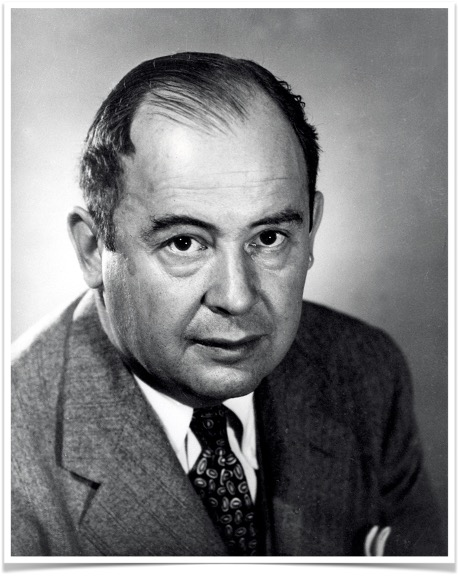
\includegraphics[align=c,height=0.49\paperheight]{L3/von-n}
    \end{column}
   \end{columns}
   \footnotetext[1]{\scriptsize You might wonder how a theorem from 1928 can use the term "Nash equilibrium," when Nash's work was published in 1950. 
   John von Neumann used different terminology and proved the theorem in a different way; however, the given presentation is probably clearer in the context of modern game theory}
  \end{frame} 
  
  \begin{frame}{Example}
   \begin{center}
   \hspace{-5em}
    \begin{game}{2}{2}[Agent 1][Agent 2]
      		\> Left   	\> Right		\\
     Up 		\> $20,-20$	\> $0,0$		\\
     Down 	\> $0,0$ 	\> $10,-10$
    \end{game}
   \end{center}
   \vspace{1 em}
   \begin{itemize}[<+->]
    \item What is maximin value of agent 1 with and without mixed strategies?
    \item What is minimax value of agent 1 with and without mixed strategies?
    \item What is NE of this game?
   \end{itemize}
  \end{frame}
  
 \section{Rationalizability} 
  \begin{frame}{Rationalizability}
   \begin{itemize}[<+->]
   \setlength{\itemsep}{1.1em}
    \item \alert{Rationalizable} strategy: \underline{Perfectly rational} agent could justifiably play it
    \begin{itemize}
     \item Best response to some beliefs about strategies of others
    \end{itemize}
    \item Agents cannot have arbitrary beliefs about other agents
    \item Agent $i$'s beliefs must take into account:
    \begin{itemize}
     \setlength{\itemsep}{1.1em}
     \item Other agents' rationality
     \item Other agents' knowledge of agent $i$'s rationality
     \item Other agents' knowledge of agent $i$'s knowledge of their rationality
     \item $\dots$ (infinite regress)
    \end{itemize}
   \end{itemize}
  \end{frame}
  
  \begin{frame}{Example: Matching Pennies}
   \begin{center}
    \hspace{-3.5em}
    \begin{game}{2}{2}
     	\> H			\> T			\\
     H	\> $-1,1$	\> $1,-1$	\\
     T	\> $1,-1$	\> $-1,1$
    \end{game}
   \end{center}
   \vspace{0.5cm}
   \begin{itemize}[<+->]
    \item Col playing H is rationalizable
    \begin{itemize}
     \item Col could believe Row plays H
    \end{itemize}
    \item Col believing that Row plays H is rationalizable
    \begin{itemize}
     \item Col could believe Row believes Col plays T
    \end{itemize}
    \item Col believing that Row believes that Col plays T is rationalizable
    \begin{itemize}
     \item Col could believe Row believes Col believes Row plays T
    \end{itemize}
    \item $\dots$
    \item In this game, all pure strategies are rationalizable
   \end{itemize}
  \end{frame}
  
  \begin{frame}{Rationalizability: Properties}
   \begin{itemizes}
    \item Nash equilibrium strategies are always rationalizable
    \item<+-> Some rationalizable strategies are not Nash
    \begin{itemize}
     \item Set of rationalizable strategies in finite games is nonempty
    \end{itemize}
    \item<+-> To find rationalizable strategies:
    \begin{itemize}
     \setlength{\itemsep}{1.1em}
     \item<+-> In \alert{2-player} games, use iterated elimination of strictly dominated strategies
     \item<+-> In \alert{$n$-player} games, iterated elimination of \alert{never-best response} strategies
     \begin{itemize}
      \item Eliminate strategies that are not optimal against any belief about others' strategies
     \end{itemize}
    \end{itemize}
   \end{itemizes}
  \end{frame}
  
  \begin{frame}{Example: 2/3-Beauty Contest Game}
   \begin{itemize}[<+->]
    \item No agent plays more than 100
    \item 2/3 of average is strictly less than 67 (100 $\times$ 2/3)
    \item Any integer $>$ 67 is never-best response to any belief about others' strategy
    \item No agent plays more than 67
    \item 2/3 of average is less than 45 (67 $\times$ 2/3)
    \item Any integer $>$ 45 is never-best response to any belief about others' strategy
    \item $\dots$
    \item Only rationalizable action is playing 1
   \end{itemize}
  \end{frame}
 
 \section{Correlated Equilibrium}
  \begin{frame}{Example: Battle of Sexes}
   \begin{center}
    \hspace{-9.8em}
    \begin{game}{2}{2}[H][W]
      	\> Football		\> Opera		\\
     F	\> $2, 1$		\> $0, 0$	\\
     O	\> $0, 0$		\> $1, 2$
    \end{game}
   \end{center}
   \vspace{1em}
   \begin{itemize}[<+->]
   	\item Unique mixed strategy NE yields each agent expected payoff of 2/3
    \item In NE, agents randomize over strategies \alert{independently}
    \item Can they both do better by coordinating?
    \item Agents can observe random coin flip and condition their strategies on its outcome
   \end{itemize}
  \end{frame}

  \begin{frame}{Example: Battle of Sexes (cont.)}
   \begin{itemize}[<+->]
   \setlength{\itemsep}{1.1em}
    \item Suppose there is \alert{publicly observable} fair coin
    \item If it is heads/tails, they both get \alert{recommendation} to go to football/opera
    \item If they see heads, they believe that the other one goes to football
    \item Going to football is best response, agents have \alert{no incentive to deviate}
    \item Similar argument can be made when they see tails
    \item Expected utilities for this play of game \alert{increases} to $(1.5, 1.5)$
   \end{itemize}
  \end{frame}
  
  \begin{frame}{Correlated Recommendations}
   \begin{itemize}[<+->]
    \setlength{\itemsep}{0.56em}
    \item Let $R=(R_1,\dots,R_n)$ be random variable taking values in $A=\prod_i A_i$
    \item Let $R$ be distributed according to $\pi \in \Delta(A)$
    \item $r = (r_1, \dots, r_n)$ is an instantiatation of $R$ and a pure strategy profile
    \item $r_i \in A_i$ is called \alert{recommendation to agent $i$}
    \item $\pi(r_i)$ represents marginal probability for $R_i = r_i$
    \item Given $r_i$, agent $i$ can use conditional probability to form beliefs others' signals
    $$\pi(r_{-i} | r_i) = \frac{\pi(r_i, r_{-i})}{\sum_{r^{\prime}_{-i}\in A_{-i}}\pi(r_i,r^{\prime}_{-i})}$$
   \end{itemize}
  \end{frame}

  \begin{frame}{Correlated Equilibrium: Formal Definition}
   \begin{itemize}[<+->]
    \item \alert{Correlated equilibrium} of finite game is joint probability distribution $\pi \in \Delta(A)$ such that if $R$ is random variable distributed according to $\pi$, then for all $i, r_i \in A_i$ with $\pi(r_i) > 0$, and $r^{\prime}_i \in A_i$
    $$
     \sum_{r_{-i} \in A_{-i}} \pi(r_{-i} \mid r_i) \left[u_i(r_i, r_{-i}) - u_i(r^{\prime}_i, r_{-i})\right]  \ge 0
    $$
    \item No agent can benefit by deviating from their recommendation, assuming that other agents follow their recommendations
   \end{itemize}
  \end{frame}

  \begin{frame}{Example: Game of Chicken}
   \begin{center}
    \hspace{-9.8em}
    \begin{game}{2}{2}[Driver 1][Driver 2]
     	\> Dare		\> Yield			\\
     D	\> $-5, -5$	\> $ 1, -1$		\\
     Y	\> $-1,  1$	\> $ 0,  0$
    \end{game}
   \end{center}
   \begin{itemize}[<+->]
    \item (D,Y) and (Y,D) are \alert{strict} pure-strategy NE
    \item Assume Driver 1 yields w.p. $p$ and Driver 2 yields w.p. $q$
    \item Using mixed equilibrium characterization, we have 
	$$ p - 5\times (1 - p) = - (1 - p) \implies p = 4/5 $$
    $$ q - 5\times (1 - q) = - (1 - q) \implies q = 4/5 $$
    \item Mixed-strategy NE utilities are $(-0.2, -0.2)$, people \alert{die} with probability $0.04$
   \end{itemize}
  \end{frame}

  \begin{frame}{Example: Game of Chicken (cont.)}
   \begin{columns}
    \begin{column}{0.6\textwidth}
      \vspace{-1em}
      \begin{itemize}[<+->]
       \item Is this correlated equilibrium?
       \item Suppose D1 gets Y recommendation 
       \item Conditional probability that D2 yields is 1/3
       \item Expected utility of Y is 1 $\times$ -2/3
       \item Expected utility of D is 1 $\times$ 1/3 - 5 $\times$ 2/3
       \item Following the recommendation is better
       \item If D1 gets D recommendation, D2 must yield
       \item Following recommendation is again better
       \item Similar analysis works for D2
       \item Expected utilizes are $(0,0)$, so nobody dies!
      \end{itemize}
    \end{column}
    \begin{column}{0.28\textwidth}
     \begin{center}
      \renewcommand{\gamestretch}{2.5}
      \vspace{-9.2em}
      \hspace{-3.2em}
      \begin{game}{2}{2}[D1][D2]
            \> D									\> Y	     						\\
        D   \> $\stackedpayoffs{-5, -5}{0\%}$		\> $\stackedpayoffs{1, -1}{40\%}$	\\
        Y   \> $\stackedpayoffs{-1,  1}{40\%}$	\> $\stackedpayoffs{0,  0}{20\%}$
      \end{game}
     \end{center}
    \end{column}
   \end{columns}
  \end{frame}

  \begin{frame}{Characterization of Correlated Equilibrium}
   \begin{itemize}[<+->] 
    \item Join distribution $\pi \in \Delta(S)$ is correlated equilibrium of finite game iff
     \begin{equation}
     \label{equ:CE}
      \sum_{r_{-i} \in A_{-i}} \pi(r) \left[u_i(r) - u_i(r^{\prime}_i, r_{-i})\right] \ge 0,\quad  \forall i, r_i, r^{\prime}_i \in A_i
     \end{equation}
    \item Proof (only for one side):
    \begin{itemize}
     \item Correlated equilibrium can be written for all $i, r_i, r^{\prime}_i \in A_i$ with $\pi(r_i) > 0$ as:
     $$
      \sum_{r_{-i} \in A_{-i}} \frac{\pi(r_i,r_{-i})}{\sum_{r^{\prime}_{-i} \in A_{-i}} \pi(r_i, r^{\prime}_{-i})} \left[u_i(r_i, r_{-i}) - u_i(r^{\prime}_i, r_{-i})\right] \ge 0
     $$
     \item Denominator does not depend on variable of sum
     \item So it can be factored and canceled
     \item If $\pi(r_i) = 0$, LHS of (\ref{equ:CE}) is zero regardless of $i$ and $r^{\prime}_i$, so equation always holds
    \end{itemize}
   \end{itemize}
  \end{frame}
  
  \begin{frame}{Acknowledgment}
   \begin{itemize}
    \setlength{\itemsep}{1em}
    \item This lecture is a slightly modified version of ones prepared by
    \begin{itemizes}
     \item Asu Ozdaglar \href{https://ocw.mit.edu/courses/electrical-engineering-and-computer-science/6-254-game-theory-with-engineering-applications-spring-2010/index.htm}{[MIT 6.254]}
     \item Vincent Conitzer \href{https://courses.cs.duke.edu/spring16/compsci590.4/}{[Duke CPS 590.4]}
    \end{itemizes}
    \item Aravind Vellora Vayalapra helped with importing slides from PowerPoint to \LaTeX
   \end{itemize}
  \end{frame}
 
\end{document}
